\section*{\centering Cronograma}

\subsection*{Integrantes}
    \begin{itemize}
        \item Oscar Martinez Barrales
        \item Oswaldo Mejia Garcia
        \item Aaron Rodrigo Ramos Reyes
        \newline
    \end{itemize}


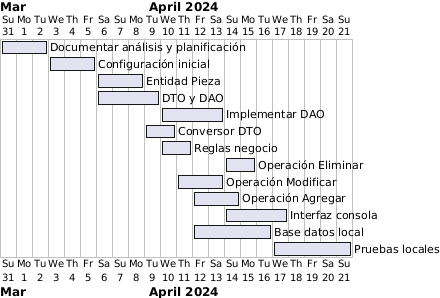
\includegraphics[width=.9\textwidth]{imag/DiagramaCronograma.png}


\subsection*{Descripción de la Imagen}


\begin{itemize}
    \item \textbf{Documentar análisis y planificación}: Crear documentación sobre los objetivos, requerimientos y planificación del proyecto.
    \item \textbf{Configuración inicial}: Preparar el entorno de desarrollo y las herramientas necesarias.
    \item \textbf{Entidad Pieza}: Modelar la entidad "Pieza" en el sistema.
    \item \textbf{DTO y DAO}: Diseñar los Data Transfer Objects (DTO) y Data Access Objects (DAO).
    \item \textbf{Implementar DAO}: Programar la capa de acceso a datos.
    \item \textbf{Conversor DTO}: Implementar conversores para transformar datos entre diferentes capas del sistema.
    \item \textbf{Reglas de negocio}: Definir e implementar las reglas que rigen la lógica del negocio.
    \item \textbf{Operación Eliminar}: Implementar la funcionalidad para eliminar datos.
    \item \textbf{Operación Modificar}: Implementar la funcionalidad para modificar datos.
    \item \textbf{Operación Agregar}: Implementar la funcionalidad para agregar nuevos datos.
    \item \textbf{Interfaz consola}: Diseñar y programar la interfaz basada en consola.
    \item \textbf{Base de datos local}: Configurar una base de datos local para el proyecto.
    \item \textbf{Pruebas locales}: Realizar pruebas para verificar la correcta funcionalidad del sistema.
\end{itemize}

\section{Asignación de Tareas}

\begin{table}[h]
    \centering
    \begin{tabular}{|c|c|}
        \hline
        \textbf{Responsable} & \textbf{Tareas Asignadas} \\
        \hline
        Aaron & Documentar análisis y planificación, Implementar DAO, Operación Eliminar, Base de datos local \\
        \hline
        Oscar & Configuración inicial, Conversor DTO, Operación Modificar, Pruebas locales \\
        \hline
        Oswaldo & Entidad Pieza, DTO y DAO, Reglas de negocio, Operación Agregar, Interfaz consola \\
        \hline
    \end{tabular}
    \caption{Distribución de tareas entre el equipo de desarrollo}
\end{table}


